% Exploratory v4 revision. Numerical claims map to eda/rebuild_v4 outputs.
% Build from D:\AEpaper with xelatex twice; author metadata awaits confirmation.
\documentclass[preprint,12pt]{elsarticle}
\usepackage{amsmath,amssymb,booktabs,array,graphicx,placeins,float,url}
\journal{Applied Energy}
\begin{document}
\begin{frontmatter}
\title{Data provenance, endpoint definitions and censoring in cross-dataset battery lifetime prediction}
\author[aff1]{[First Author]\corref{cor1}}
\ead{[corresponding.author@email]}
\cortext[cor1]{Corresponding author}
\affiliation[aff1]{organization={[Department, University]}, country={[Country]}}

\begin{abstract}
Battery-life prediction may not transfer when public archives differ in capacity semantics, observation schedules and end-of-life ascertainment. We audited six sources and retained 429 cells and 340,838 verified cycle records. End of life was the first of three consecutive observed state-of-health records at or below 0.8; right censoring was retained. At cycle 100, 376 cells (228 observed events) entered source-held-out folds. Five survival approaches were fitted to remaining life after the landmark with source-only tuning. Source-specific integrated inverse-censoring-weighted Brier scores had no universal winner: the survival forest scored 0.139 on MIT and 0.155 on TJU, XGBoost accelerated failure time (AFT) scored 0.055 on XJTU and 0.117 on HUST, and an unfeatured source Kaplan--Meier baseline scored 0.040 on nine CALCE cells. NASA supported only one scoring horizon. Within-source and event-only controls showed no uniform advantage for censor-aware training, while endpoint and source-correction audits changed errors in both directions. At a 20\% target-cell budget, average target-shift improvement was confined to CALCE, which had two calibration cells; TJU improved in 13/30 seed-0 draws. An event-only finite-quantile calculation gave a 5.22\% chance of obtaining 19 event labels in TJU, which is not a coverage result. These findings delimit retrospective cross-source transfer claims.
\end{abstract}
\begin{keyword}
battery cycle life \sep cross-source validation \sep right censoring \sep survival analysis \sep endpoint sensitivity \sep probability recalibration
\end{keyword}
\end{frontmatter}

\section{Introduction}
Battery-life models are often evaluated within one measurement protocol. A model deployed on a different archive must also face differences in capacity definition, measurement frequency, chemistry, cycling policy, and censoring. Apparent accuracy can change when an isolated capacity drop is called an end-of-life (EOL) event or when only completed lifetimes are scored. Published early-life predictors and recent physics-informed and cross-domain models motivate a source-held-out evaluation \citep{severson2019,wang2024pin,tang2024ae,ledeng2026,zhu2026lake}. An auditable comparison needs a common prediction time, endpoint, and evaluation rule.

We ask how source records, endpoint definitions, and censoring affect lifetime predictions across archives. Our contributions are (i) a traceable six-source corpus and endpoint audit; (ii) a landmark-consistent comparison of five survival approaches under source-only model selection; and (iii) paired analyses of source correction, endpoint sensitivity, within-source training, event-only regression, target-label budgets, and recalibration. This is a retrospective cell-level analysis. It does not establish prospective battery energy storage system control benefits.

\section{Materials and methods}
\subsection{Source records and endpoint}
The verified corpus contains 124 MIT, 55 XJTU, 130 TJU, 34 unique NASA, 9 CALCE, and 77 HUST cells. The source publications and repositories are cited separately \citep{severson2019,wang2024pin,wang2024dataset,zhu2022tju,zhu2022dataset,saha2007,calce2026,ma2022hust,ma2022hustdata}. Provenance files identify the selected raw records, hashes, parser decisions, and corrections. In particular, NASA cathode chemistry is not certified by the available local metadata; CALCE CS/CX and K2 subsets have different reported cathodes; TJU mAh values were converted to Ah and partial-counter records were excluded under the documented rule. Raw archives remain with their providers; the processed table and audit manifest are versioned locally. Figure~\ref{fig:cohort} shows source counts and the cycle-100 landmark cohort; Supplementary file S1 describes recorded chemistry, temperature, protocol grouping, and observation density.

Let $Q_j(c)$ denote a valid capacity observation for cell $j$ at cycle $c$. We define $\mathrm{SOH}_j(c)=Q_j(c)/Q_j(1)$. The primary EOL time is the first of three consecutive \emph{observed records} with SOH $\leq0.8$. A record is not required to be at an adjacent integer cycle. Cells without this run are censored at the last valid observation. One- and five-record definitions are sensitivity analyses; changing the rule changes the outcome, not merely its estimated error. At landmark $L\in\{50,100\}$, only cells observed event-free past $L$ and only capacity records available by $L$ enter the predictor. The cycle-100 cohort has 376 cells, 228 events, and 148 censored outcomes; the cycle-50 cohort has 379 cells, 230 events, and 149 censored outcomes. Of the 34 unique NASA cells, 11 had reached the observed-record endpoint by cycle 100 and 15 had no follow-up after cycle 100, leaving eight eligible cells. This attrition is a landmark eligibility result, not loss of source files.

\begin{figure}[htbp]\centering
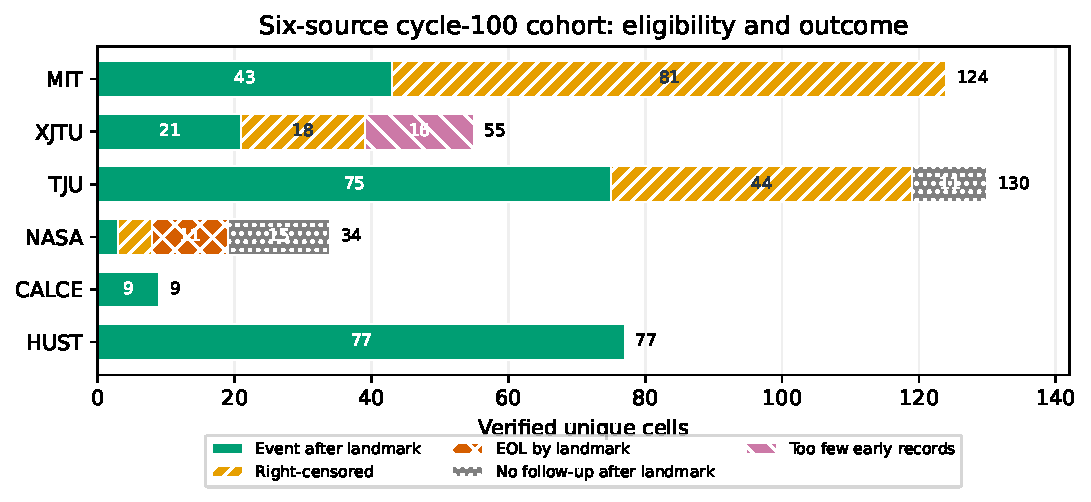
\includegraphics[width=0.88\linewidth]{figures_v4/fig_v4_source_cohort.pdf}
\caption{Source-level counts of verified unique cells at cycle 100. Events and right-censored outcomes are among eligible cells; other segments identify the exclusive landmark-exclusion reasons. Source totals appear at right. Exclusions are based on the recorded endpoint and follow-up, not missing archives.}\label{fig:cohort}
\end{figure}

\subsection{Landmark-consistent survival analysis}
For an eligible cell we model remaining life $R=T-L$, with residual follow-up $Y=\min(T,C)-L>0$ and event indicator $\Delta=I(T\leq C)$. An event contributes $f_R(Y\mid x)$ to a continuous likelihood and a censored cell contributes $S_R(Y\mid x)$. For the lognormal AFT models, $\log R=\mu(x)+\sigma Z$, $Z\sim N(0,1)$, hence the absolute-cycle event risk at $t>L$ is
\begin{equation}
F(t\mid x,T>L)=\Phi\!\left(\frac{\log(t-L)-\mu(x)}{\sigma}\right).
\end{equation}
The reported median total lifetime is $L+\exp\{\mu(x)\}$. This parameterization uses the same residual time axis for fitting, prediction, and scoring. Eight capacity-derived features are used: initial capacity, landmark SOH, early slope, two observed drops, SOH variability, and two recovery measures. The redundant feature $1-\mathrm{SOH}(L)$ was removed because it duplicates an existing column exactly. Imputation and scaling are learned inside each training fold.

We compare an unfeatured source Kaplan--Meier (KM) model \citep{kaplan1958}, regularized lognormal AFT, regularized Cox regression \citep{cox1972}, random survival forest \citep{ishwaran2008}, and XGBoost AFT. Every outer fold holds out one source; candidate parameters are selected by an inner leave-one-source-out analysis among the other five sources. No held-out outcome selects the model or parameter. The machine-readable configuration records candidate sets, fixed training budgets, predictions, and convergence status. XGBoost AFT alone is refitted with 20 seeds after source-only selection; these are descriptive training-sensitivity runs.

At absolute cycles 125, 250, 500, 750, 1000, 1500, and 2000, we compute inverse-probability-of-censoring-weighted (IPCW) Brier scores using the held-out source's censoring KM estimate \citep{gerds2006}. Unsupported horizons are left unavailable. Integrated Brier scores are trapezoidal summaries over the supported horizons \emph{within the same held-out source}; because support ranges vary by source, we do not pool these integrals into a global model ranking. Harrell concordance \citep{harrell1982} and observed-event median absolute percentage error (MedAPE) are secondary measures. IPCW interpretation assumes independent censoring under the available information, which cannot be established from these archives alone.

\subsection{Controlled sensitivity and target adaptation}
For endpoint sensitivity, we restrict all one-, three-, and five-record rules to cells eligible under every rule at each landmark. The original three-record source-selected parameters are held fixed and Cox and XGBoost AFT are refitted for each rule. Their integrated Brier scores are recomputed on the intersection of supported horizons across the three rules within each source. We separately compare training before and after verified source correction while retaining identical verified test labels and cells; this isolates the effect of changed training records, not a changed test reference.

Two exploratory controls address training-domain and event-selection sensitivity. Within each target source, stratified cell-level three-fold validation (NASA and CALCE) or five-fold validation (other sources) yields one out-of-fold XGBoost AFT prediction per cell; the scale is the parameter previously selected without that source's labels. This arm uses labels from other cells in the target source, while the frozen source-held-out AFT uses none. The event-only arm trains XGBoost squared-error regression of log remaining life on observed source events, with the same eight features, tree settings and 300 boosting rounds as the source AFT, and tests on the same held-out cells. For Brier scoring, its point output is assigned the source-selected AFT scale as a specified lognormal risk proxy; this arm does not independently estimate a probability distribution. Ten alternative within-source partitions and 20 paired regression/AFT training seeds describe sensitivity, not independent replications.

For XJTU and TJU, the available within-source group labels permit another out-of-group control: XJTU batches 1--4 and TJU's three battery subsets are each held out in turn, with AFT trained on the other groups of that source. The pooled predictions are scored on the same source cells as the zero-shot model. TJU subset identity combines protocol and chemistry, so its contrast does not isolate either factor. MIT and HUST lack a usable group distinction in the current table, and NASA is too small for this control.

For exploratory target adaptation, frozen source-held-out XGBoost AFT predictions are randomly divided without event stratification into $m=\lceil pn\rceil$ calibration cells and the remaining evaluation cells, for $p\in\{0.10,0.20,0.40\}$. Thirty fixed draws are used per budget. A target calibration set fits a bounded log-remaining-life shift $\delta$ by censored likelihood plus $\delta^2/(2\tau^2)$; the AFT scale stays fixed. The prior log-shift SD $\tau$ is selected from $\{0.25,0.5,1.0\}$ separately for each outer fold using ten random 20\% calibration/evaluation draws in each of its five source-validation domains. The selection minimizes mean evaluation censored negative log-likelihood without using the outer target labels; all cycle-100 folds select $\tau=1.0$. We compare shifted and unshifted probabilities on identical held-out cells and horizons. All 20 AFT training seeds are crossed with the same 30 target draws at the 20\% budget. These overlapping evaluations are sensitivity distributions, not 600 independent experiments or confidence intervals. Brier changes assess prediction error and cannot alone prove probability calibration.

For a separate event-only absolute-residual split-conformal feasibility calculation, a finite empirical 95\% quantile needs at least 19 exchangeable event residuals because $\lceil(n_{\rm cal}+1)0.95\rceil\leq n_{\rm cal}$ first holds at $n_{\rm cal}=19$ \citep{angelopoulos2021}. We compute the exact hypergeometric probability of reaching that count under a random target-cell allocation. The calculation does not establish interval coverage for the full censored target population.

\section{Results}
\subsection{Source-held-out model comparison}
Table~\ref{tab:main} reports cycle-100 integrated IPCW Brier scores together with XGBoost AFT discrimination and observed-event error. The supported grid is common to all five models within each listed source. A model ranking does not generalize across sources: the forest has the smallest score on MIT and TJU, XGBoost AFT on XJTU and HUST, and source KM on CALCE. On CALCE, the unfeatured KM score is 0.040 versus 0.254 for XGBoost AFT; only nine cells are available. NASA has eight eligible cells and three observed events, and only cycle 125 supports scoring, so no integrated score is reported. Harrell C for XGBoost AFT ranges from 0.491 on XJTU to 0.778 on NASA and CALCE, but the NASA value is based on only eight cells and three observed events. MedAPE is computed only on observed events and can rank models differently from the Brier score.

\begin{table}[htbp]
\caption{Cycle-100 source-held-out integrated IPCW Brier score (lower is better), plus XGBoost AFT Harrell C and event-only MedAPE. Each source uses its supported cycle grid; model Brier comparisons are paired within a row. NASA supports only one horizon and has no integral. Harrell C and MedAPE use different evaluation targets from Brier.}
\label{tab:main}\centering\scriptsize\setlength{\tabcolsep}{2.6pt}
\resizebox{\linewidth}{!}{\begin{tabular}{@{}lrrccccccc@{}}\toprule
Source & Cells & Events & Source KM & Lognormal AFT & Cox & Forest & XGBoost AFT & XGB C & XGB MedAPE (\%)\\\midrule
MIT & 124 & 43 & 0.163 & 0.175 & 0.185 & \textbf{0.139} & 0.145 & 0.685 & 198.3\\
XJTU & 39 & 21 & 0.058 & 0.084 & 0.078 & 0.065 & \textbf{0.055} & 0.491 & 190.5\\
TJU & 119 & 75 & 0.325 & 0.208 & 0.180 & \textbf{0.155} & 0.190 & 0.538 & 49.2\\
NASA & 8 & 3 & NA & NA & NA & NA & NA & 0.778 & 201.4\\
CALCE & 9 & 9 & \textbf{0.040} & 0.154 & 0.102 & 0.177 & 0.254 & 0.778 & 49.2\\
HUST & 77 & 77 & 0.259 & 0.179 & 0.168 & 0.307 & \textbf{0.117} & 0.656 & 50.3\\\bottomrule
\end{tabular}}
\end{table}
\begin{table}[htbp]
\caption{Cycle-100 exploratory controls on identical target cells and supported horizons. The within-source arm uses target-source training labels and has a different training-set size. Event-only regression uses only observed events for supervised fitting and an AFT scale for its probability proxy. Lower integrated Brier score is better; NASA has only one supported horizon.}
\label{tab:controls}\centering\scriptsize\setlength{\tabcolsep}{4pt}
\begin{tabular}{@{}lrrccc@{}}\toprule
Target source & Cells & Events & Source AFT & Within-source AFT & Event-only regression\\\midrule
MIT & 124 & 43 & 0.145 & 0.060 & 0.141\\
XJTU & 39 & 21 & 0.055 & 0.087 & 0.062\\
TJU & 119 & 75 & 0.190 & 0.165 & 0.144\\
NASA & 8 & 3 & NA & NA & NA\\
CALCE & 9 & 9 & 0.254 & 0.092 & 0.282\\
HUST & 77 & 77 & 0.117 & 0.121 & 0.436\\\bottomrule
\end{tabular}
\end{table}
Table~\ref{tab:controls} shows that within-source AFT has a lower score on MIT, TJU and CALCE, but not XJTU or HUST. Under ten alternative partition seeds, each of these directions persists; this does not remove small-source uncertainty or the difference in label access and training size. Event-only regression scores below source AFT on TJU in all 20 paired training seeds, above it on HUST in all 20, and changes direction across seeds on MIT, XJTU and CALCE. At cycle 50, XJTU reverses its within-source comparison (0.074 versus 0.387), demonstrating landmark dependence. Thus neither in-domain fitting nor censor-aware training yields a universal advantage in this corpus. The event-only Brier contrast also depends on the stated scale borrowed from source AFT.

Holding out whole protocol groups changes this picture again. At cycle 100, XJTU's pooled group-held-out score is 0.058 versus 0.055 for the source-held-out model, and TJU's is 0.247 versus 0.190. At cycle 50, XJTU's group-held-out score is 0.079 versus 0.387, while TJU's is 0.289 versus 0.222. These source-level pooled comparisons use the same cells and supported horizons but different training sample sizes; XJTU batch 2 has only one observed event among its 15 test cells, and TJU group identity is chemistry-confounded. The results do not establish a general cross-protocol transfer effect. Figure~\ref{fig:benchmark} displays the five-model source comparison.
\begin{figure}[H]\centering
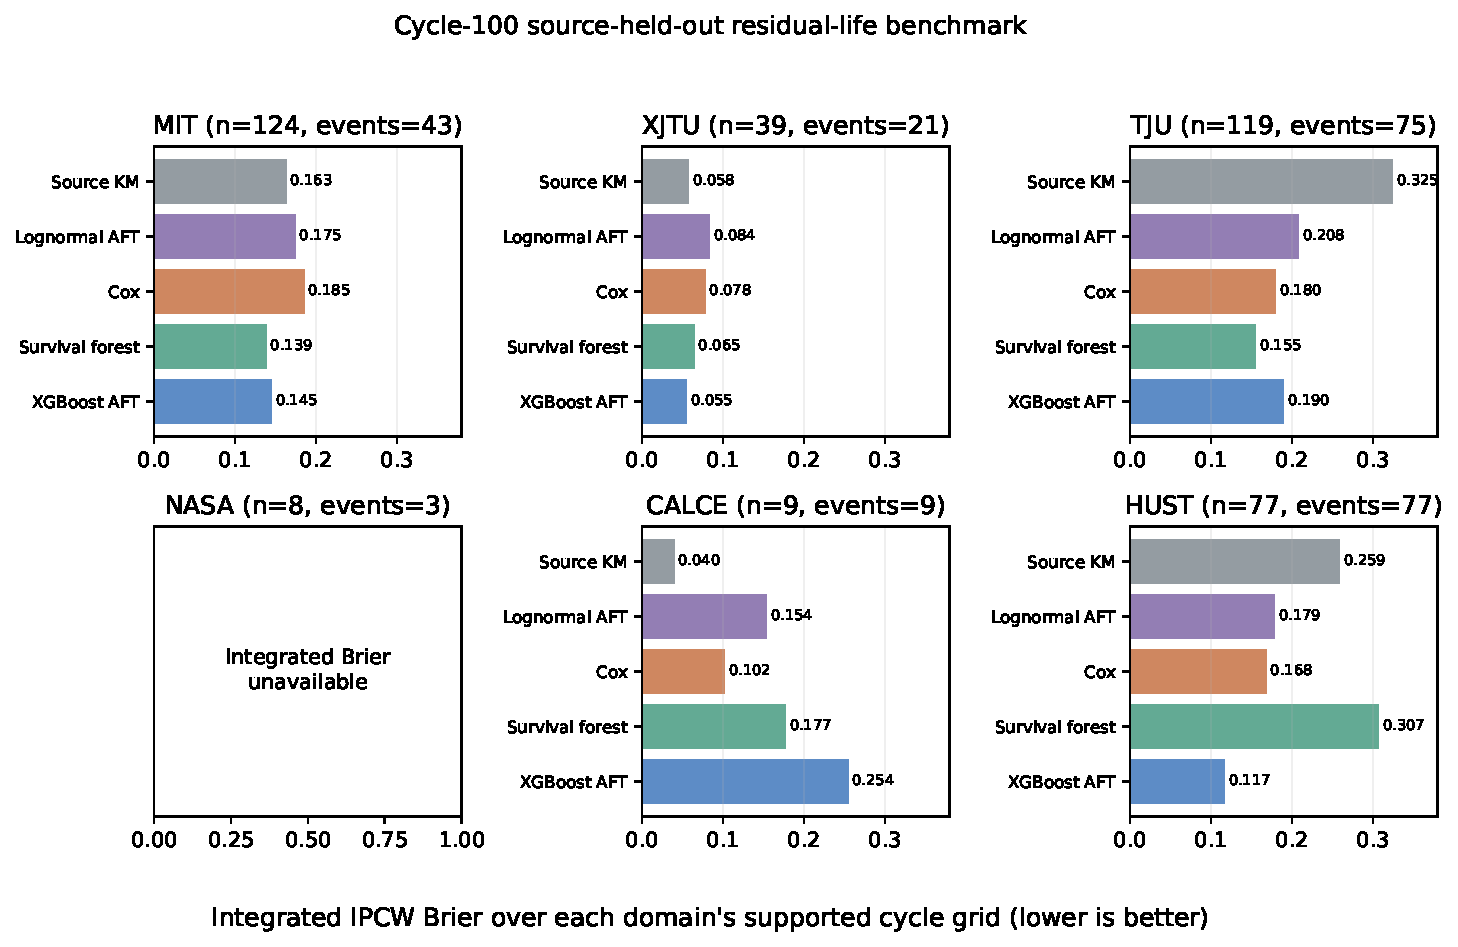
\includegraphics[width=0.94\linewidth]{figures_v4/fig_v4_benchmark_brier.pdf}
\caption{Five-model cycle-100 benchmark. Each panel compares models on the same source-specific supported horizons. The NASA integral is unavailable.}\label{fig:benchmark}
\end{figure}
The time-specific risk audit also shows that a small integrated score does not establish reliable event probabilities. At cycle 500, CALCE's mean XGBoost AFT event risk is 0.672 versus held-out KM risk 0.111; at cycle 2000, HUST's values are 0.451 and 0.896. These are fold-level comparisons at supported horizons, not individual calibration curves. Figure~\ref{fig:risk} retains every supported cycle-100 horizon, including the single NASA point.
\begin{figure}[H]\centering
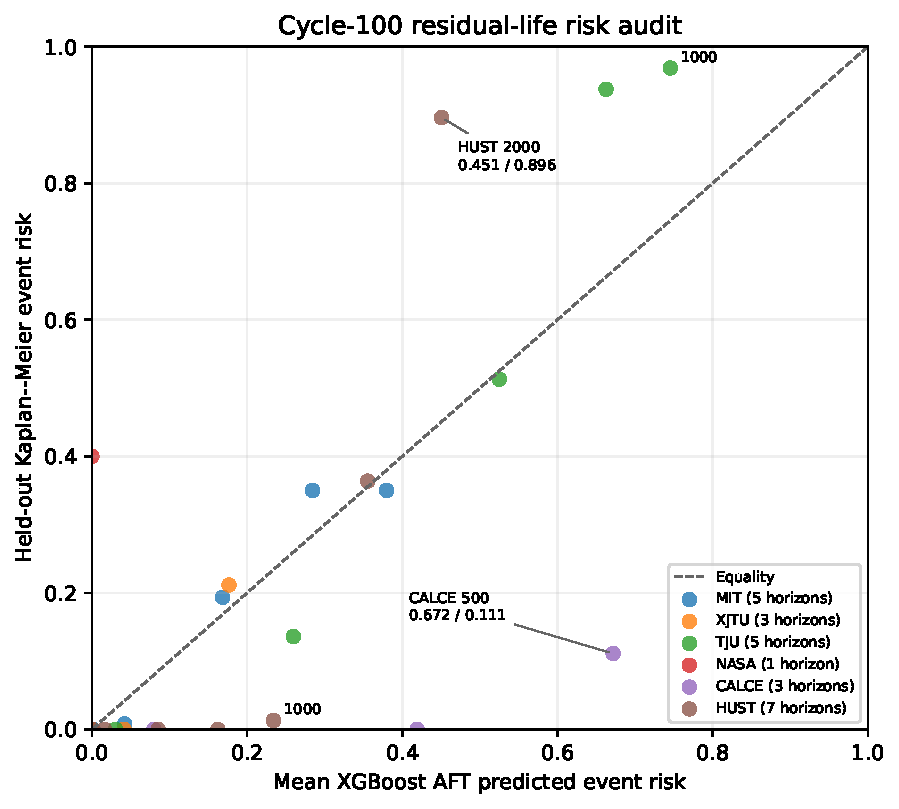
\includegraphics[width=0.68\linewidth]{figures_v4/fig_v4_survival_calibration.pdf}
\caption{Mean XGBoost AFT event risk against held-out KM event risk at supported cycle-100 horizons. The dashed line indicates equality. Labels identify selected absolute cycle horizons. NASA has one supported point.}\label{fig:risk}
\end{figure}

\subsection{Endpoint and source-correction sensitivity}
At cycle 100, the cohort eligible under all endpoint rules contains 374 cells, two fewer than the main three-record cohort. On this paired cohort and shared horizon grid, the XGBoost AFT score for XJTU changes from 0.091 under one observed low-SOH record to 0.059 under three and 0.049 under five; observed events change from 24 to 21 to 16. Cox changes from 0.290 to 0.082 to 0.071 in the same comparison. These values describe different outcomes and should not be interpreted as evidence that the five-record rule is more accurate. NASA remains unsupported for an integral. Figure~\ref{fig:endpoint} gives all domains, with common cells and horizons within each panel.

\begin{figure}[htbp]\centering
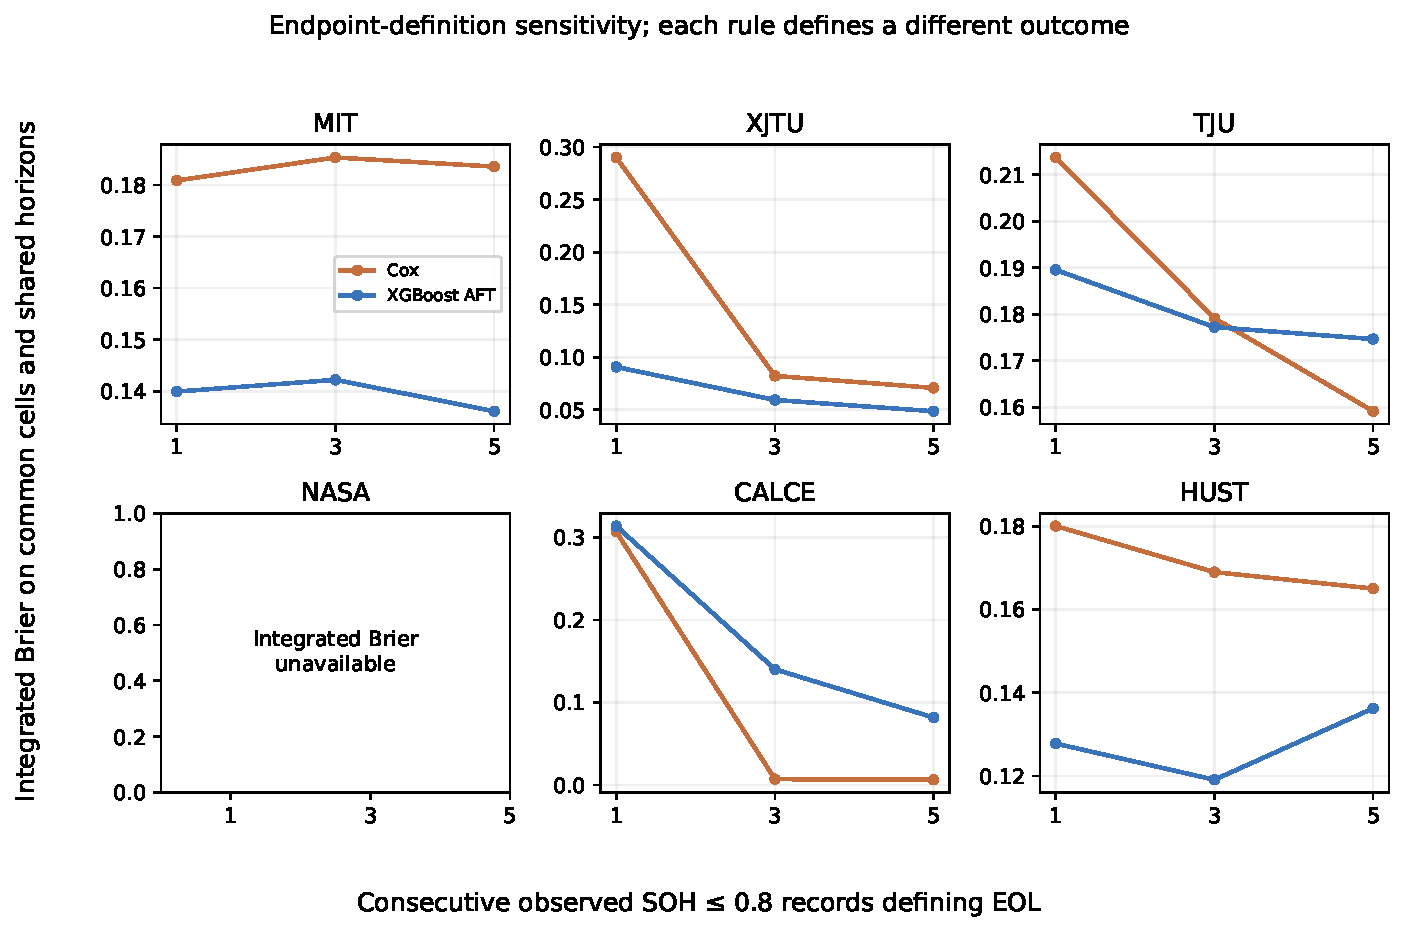
\includegraphics[width=0.94\linewidth]{figures_v4/fig_v4_endpoint_model_sensitivity.pdf}
\caption{Endpoint sensitivity for Cox and XGBoost AFT at cycle 100. Cell cohorts and scoring horizons are held common across endpoint rules within each source; changing the endpoint still changes the prediction target. Panel vertical scales differ.}\label{fig:endpoint}
\end{figure}

Rebuilding source training features from the verified records changes model error in both directions on the fixed verified test reference (Figure~\ref{fig:correction}). For XGBoost AFT, HUST integrated Brier decreases from 0.132 to 0.117, whereas CALCE increases from 0.194 to 0.254. These changes are not a causal estimate of one individual correction: multiple source-training records can change together, and tiny target folds amplify variation. The controlled paired outputs preserve each prediction and cohort.
\begin{figure}[htbp]\centering
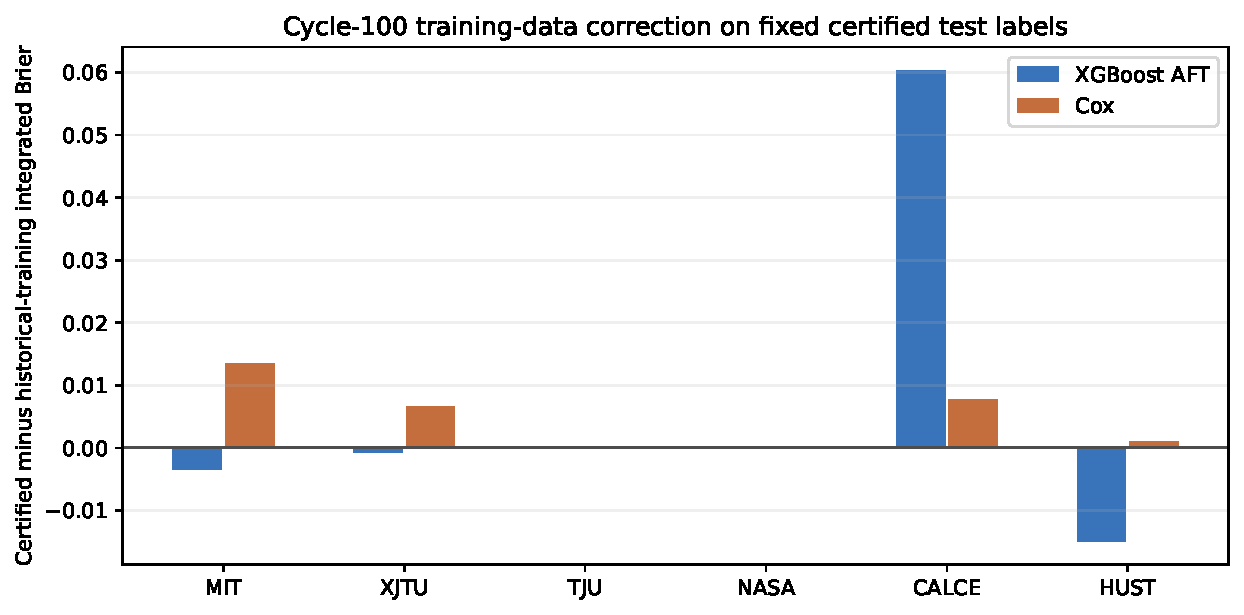
\includegraphics[width=0.82\linewidth]{figures_v4/fig_v4_source_correction.pdf}
\caption{Verified-minus-historical-training integrated Brier score at cycle 100 on identical verified test labels. Negative values favor the corrected training table.}\label{fig:correction}
\end{figure}
\FloatBarrier

\subsection{Target labels and finite-quantile feasibility}
At the 20\% budget, calibration cell counts are 25 MIT, 8 XJTU, 24 TJU, 2 NASA, 2 CALCE, and 16 HUST. For the seed-0 model, the probability shift improves the paired integrated Brier score in 5/30, 6/30, 13/30, unavailable, 29/30, and 0/30 random draws, respectively (Figure~\ref{fig:recal}). For the full crossed 20-seed/30-draw analysis, the mean paired score differences (shifted minus baseline) are $+0.0031$ MIT, $+0.0076$ XJTU, $+0.0040$ TJU, unavailable NASA, $-0.0757$ CALCE, and $+0.0079$ HUST. CALCE has only two calibration cells, so its apparently consistent gain is fragile evidence for a deployment rule. The repeated draws reuse target cells, and the 600 paired results per source do not increase its independent sample size.

\begin{figure}[htbp]\centering
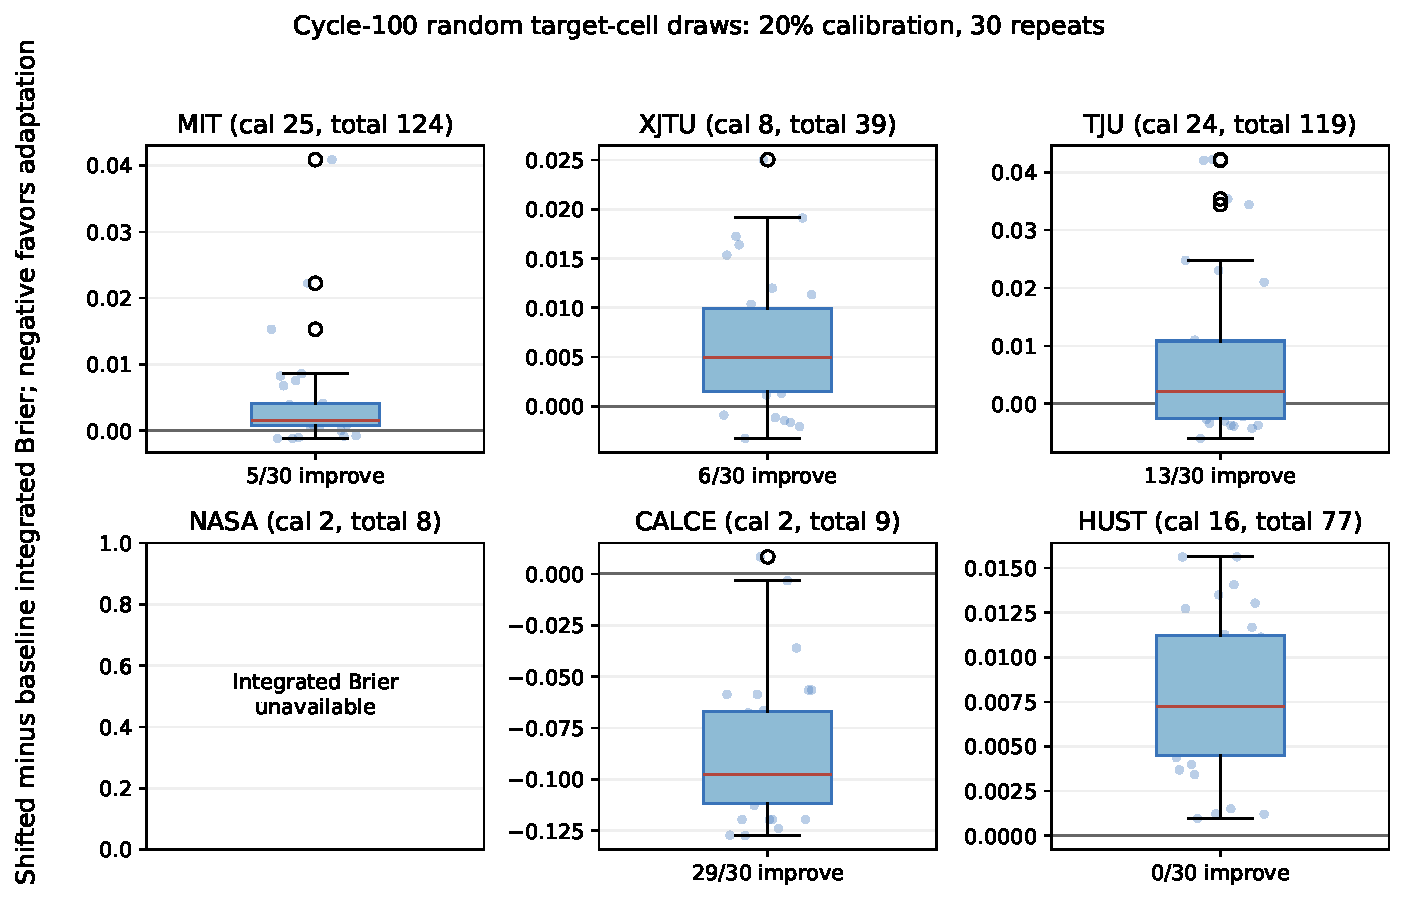
\includegraphics[width=0.94\linewidth]{figures_v4/fig_v4_target_recalibration.pdf}
\caption{Seed-0 paired integrated Brier differences after a one-parameter target shift at the cycle-100, 20\% calibration budget. Thirty ordinary random draws are shown; negative values favor the shift. The panels have different vertical scales; NASA lacks an integrated score.}\label{fig:recal}
\end{figure}

For the specified event-only finite-quantile construction, the random 20\% budget gives a 5.22\% chance of at least 19 event labels in TJU (24 calibration cells drawn from 119, including 75 observed events), and approximately $2.75\times10^{-6}$ in MIT (25 drawn from 124, including 43 observed events). The other four sources cannot reach 19 event labels with their 20\% cell budgets. This count analysis does not estimate a conformal interval or demonstrate nominal 95\% coverage under censoring.

\section{Discussion}
Three findings limit a simple transfer narrative. First, the same verified corpus and landmark task produce source-dependent rankings across five survival model families; a feature-free baseline can outperform feature models on a very small source. The paired training-domain and event-only controls also change direction across sources and landmarks. Second, endpoint rules and source correction can materially change reported scores, including directions that are unfavorable to the revised training data. Third, target probability shifts are model-, source-, and sampling-dependent; repeated seeds and overlapping splits reveal variation but do not create new independent cells.

The study's main methodological repair is the consistent remaining-life axis for landmark AFT likelihood and event probabilities. The previous total-life fit followed by a conditional survival transformation was not the likelihood used to fit the selected cohort. The current model uses $R=T-L$ throughout, and independent numerical checks compare its predicted probabilities with a separate lognormal implementation. The resulting scores supersede the earlier v3 AFT and target-recalibration numbers.

The six sources differ in chemistry, cycling, temperature, record density and observation length, and source identity confounds many of these attributes. The sample is too small to isolate causal effects of each attribute. Right-censoring weights rely on an assumption that may fail if cell testing stopped for performance-related reasons. The endpoint is defined by observed low-capacity runs and its event timestamp is retrospectively assigned to the first record in the run; a prospective alarm would only be available after the confirming record. NASA and CALCE have especially limited cells, and their estimates should be treated as case-specific. No cell-level prediction was mapped to a validated storage dispatch decision in this analysis.

\section{Conclusion}
An audited six-source battery corpus supports a landmark-consistent, censoring-aware comparison but does not support a universal battery-life transfer claim. Five model families yield different winners by source; within-source fitting and event-only regression do not show a uniform advantage under the paired exploratory controls; endpoint and source-record choices shift results; and a simple target probability correction is not reliably beneficial across domains. An event-only 95\% finite-quantile count is rarely available under a random 20\% label budget and cannot certify coverage for censored cells. The result is a reproducible account of transfer limits and data-definition sensitivity, pending independent external and prospective validation.

\section*{Data availability statement}
The source archives remain with their original providers. The local reproducibility package contains processed tables, source-hash manifests, scripts, fold predictions, configurations, and v4 figures under \texttt{eda/rebuild\_v4}. No public repository or DOI has yet been assigned; these details must be completed before submission.

\section*{Declaration of competing interest}
To be completed and approved by all authors before submission.
\section*{CRediT authorship contribution statement}
To be completed from the actual author roles before submission.
\section*{Funding}
To be completed from verified funding records before submission.
\section*{Acknowledgments}
The authors acknowledge the public dataset providers.
\section*{Declaration of generative AI and AI-assisted technologies in the manuscript preparation process}
During the preparation of this work, ChatGPT/Codex was used to assist with prose editing, consistency checks, and preparation of the graphical-abstract layout. The authors reviewed and edited the output as needed and take full responsibility for the content of the published article.
% References used in this revision; dataset reuse and claim support require final review.

\begin{thebibliography}{99}

\bibitem[Severson et~al.(2019)]{severson2019}
Severson, K.~A., Attia, P.~M., Jin, N., Perkins, N., Jiang, B., Yang, Z., et~al. (2019). Data-driven prediction of battery cycle life before capacity degradation. \textit{Nature Energy}, \textit{4}(5), 383--391. \url{https://doi.org/10.1038/s41560-019-0356-8}

\bibitem[Wang et~al.(2024)]{wang2024pin}
Wang, F., Zhai, Z., Zhao, Z., Di, Y., \& Chen, X. (2024). Physics-informed neural network for lithium-ion battery degradation stable modeling and prognosis. \textit{Nature Communications}, \textit{15}, 4332. \url{https://doi.org/10.1038/s41467-024-48779-z}

\bibitem[Tang et~al.(2024)]{tang2024ae}
Tang, A., Xu, Y., Hu, Y., Tian, J., Nie, Y., Yan, F., Tan, Y., \& Yu, Q. (2024). Battery state of health estimation under dynamic operations with physics-driven deep learning. \textit{Applied Energy}, \textit{370}, 123632. \url{https://doi.org/10.1016/j.apenergy.2024.123632}

\bibitem[Le et~al.(2026)]{ledeng2026}
Le, H., Deng, W., Nguyen, K.~T.~P., Medjaher, K., Gogu, C., \& Wu, D. (2026). Physics-informed transfer learning by embedding physics into activation functions: An application in battery health management. \textit{Applied Energy}, \textit{406}, 127161. \url{https://doi.org/10.1016/j.apenergy.2025.127161}

\bibitem[Zhu et~al.(2026)]{zhu2026lake}
Zhu, T., Wang, H., \& Wen, Y. (2026). BatteryLake: Agentic, physics-grounded curation of heterogeneous battery aging data and benchmarking. \textit{arXiv preprint arXiv:2607.09762}. \url{https://doi.org/10.48550/arXiv.2607.09762}

\bibitem[Wang(2024)]{wang2024dataset}
Wang, F. (2024). Project -- physics-informed neural network for lithium-ion battery degradation stable modeling and prognosis [Dataset]. Zenodo. \url{https://doi.org/10.5281/zenodo.10963339}

\bibitem[Zhu et~al.(2022)]{zhu2022tju}
Zhu, J., Wang, Y., Huang, Y., et~al. (2022). Data-driven capacity estimation of commercial lithium-ion batteries from voltage relaxation. \textit{Nature Communications}, \textit{13}, 2261. \url{https://doi.org/10.1038/s41467-022-29837-w}

\bibitem[Zhu et~al.(2022)]{zhu2022dataset}
Zhu, J., Wang, Y., Huang, Y., et~al. (2022). Data-driven capacity estimation of commercial lithium-ion batteries from voltage relaxation [Dataset]. Zenodo. \url{https://doi.org/10.5281/zenodo.6405084}

\bibitem[Saha and Goebel(2007)]{saha2007}
Saha, B., \& Goebel, K. (2007). Battery data set. \textit{NASA Ames Prognostics Data Repository}. NASA Ames Research Center, Moffett Field, CA. \url{http://ti.arc.nasa.gov/project/prognostic-data-repository}

\bibitem[CALCE(2026)]{calce2026}
Center for Advanced Life Cycle Engineering (CALCE). (2026). Battery research data. University of Maryland. \url{https://calce.umd.edu/data} (accessed 30 September 2026).

\bibitem[Ma et~al.(2022)]{ma2022hust}
Ma, G., Xu, S., Jiang, B., et~al. (2022). Real-time personalized health status prediction of lithium-ion batteries using deep transfer learning. \textit{Energy \& Environmental Science}, \textit{15}, 4083--4094. \url{https://doi.org/10.1039/D2EE01676A}

\bibitem[Ma(2022)]{ma2022hustdata}
Ma, G. (2022). The dataset for: Real-time personalized health status prediction of lithium-ion batteries using deep transfer learning [Dataset, version 2]. Mendeley Data. \url{https://doi.org/10.17632/nsc7hnsg4s.2}

\bibitem[Kaplan and Meier(1958)]{kaplan1958}
Kaplan, E.~L., \& Meier, P. (1958). Nonparametric estimation from incomplete observations. \textit{Journal of the American Statistical Association}, \textit{53}(282), 457--481. \url{https://doi.org/10.1080/01621459.1958.10501452}

\bibitem[Cox(1972)]{cox1972}
Cox, D.~R. (1972). Regression models and life-tables. \textit{Journal of the Royal Statistical Society: Series B (Methodological)}, \textit{34}(2), 187--202. \url{https://doi.org/10.1111/j.2517-6161.1972.tb00899.x}

\bibitem[Ishwaran et~al.(2008)]{ishwaran2008}
Ishwaran, H., Kogalur, U.~B., Blackstone, E.~H., \& Lauer, M.~S. (2008). Random survival forests. \textit{The Annals of Applied Statistics}, \textit{2}(3), 841--860. \url{https://doi.org/10.1214/08-AOAS169}

\bibitem[Gerds and Schumacher(2006)]{gerds2006}
Gerds, T.~A., \& Schumacher, M. (2006). Consistent estimation of the expected Brier score in general survival models with right-censored event times. \textit{Biometrical Journal}, \textit{48}(6), 1029--1040. \url{https://doi.org/10.1002/bimj.200610301}

\bibitem[Harrell et~al.(1982)]{harrell1982}
Harrell, F.~E., Califf, R.~M., Pryor, D.~B., Lee, K.~L., \& Rosati, R.~A. (1982). Evaluating the yield of medical tests. \textit{JAMA}, \textit{247}(18), 2543--2546. \url{https://doi.org/10.1001/jama.1982.03320430047030}

\bibitem[Angelopoulos and Bates(2021)]{angelopoulos2021}
Angelopoulos, A.~N., \& Bates, S. (2021). A gentle introduction to conformal prediction and distribution-free uncertainty quantification. \textit{arXiv preprint arXiv:2107.07511}. \url{https://doi.org/10.48550/arXiv.2107.07511}

\end{thebibliography}
\end{document}
